As mentioned in \Cref{chapter:introduction} and \Cref{chapter:related_work}, this thesis focuses on comparing different aspects of Blockchain-based Federated Learning, such as the impact of specific properties of the Blockchain platform the system runs on, and aspects of the Federated Learning process. This chapter gives an overview of the fundamental concepts and the techniques selected for some of the properties that will be compared.

\section{Machine Learning}\label{background:machine_learning}

Machine Learning is a sub-field of Artificial Intelligence that builds models based on statistical and algorithmic concepts in order to detect relevant patterns based on prior experience \cite{geron_2019}. This models learn and adapt without explicit instructions when given new data during a process called training. The data is usually structured as vectors in a multi-dimensional space, such that each vector is an \textit{instance} and each dimension is a \textit{feature}.

There are three main categories of ML algorithms: \textit{supervised learning}, \textit{unsupervised learning} and \textit{reinforcement learning} \cite{geron_2019}. Each category performs different types of tasks on different types of data. This study focuses only on classification problems in supervised learning settings.

In supervised learning, algorithms build mathematical models using a set of input samples, which are vectors from a feature space, and expected outputs for each sample. This type of data is known as labeled data, as there is a label for each sample. During training, algorithms provide the model with the input samples and improve the model by comparing its output with the expected outputs. Supervised learning problems can be divided into \textit{regression problems}, if the output is a continuous variable, or \textit{classification problems}, if the output is a discreet variable.

\section{Federated Learning}\label{background:federated_learning}

Federated Learning is a ML technique where different clients collaboratively train a model under the supervision of a centralized orchestrator. Clients are distributed heterogeneous devices with their own computing resources and they are responsible for producing and maintaining their own data \cite{9084352}. The data is assumed to be non independent or non identically distributed (\textit{non-iid}).

Since clients are heterogeneous and distributed, different communication costs and response times are normal. In addition, some clients may operate under constrained networks with either low or limited bandwidth. Therefore, it is important that new FL techniques ensure that communication and resource usage is minimized.

During the training process, the raw data never leaves the clients and only a representation of the model, such as model weights, is exchanged with the server in order to compute the global model. However, model weights can be target of inference attacks and leak secret information \cite{10.1145/3298981}.  Consequently, new innovations must be compatible with techniques that guarantee privacy, such as differential privacy, homomorphic encryption, secure multiparty computation or other cryptographic protocols.

After each round of training, the central orchestrator aggregates the local updates. Usually, this is done using a formula known as Federated Averaging (\textit{FedAvg}) \cite{10.48550/arxiv.1602.05629}, which calculates the weighted average of all clients $k \in K$ weights $w^k$:

\begin{equation}
w_{t+1} = \sum_{k \in K} \frac{n_k}{n} w_{t+1}^k
\end{equation} \label{eq:fedavg}

Where $n_k$ is the number of samples that the client $k$ used to train and $w_{t+1}^k$ the weights of client $k$ at round $t+1$.

\subsection{Architectures of Federated Learning}\label{background:archfl}

Federated Learning can be broadly divided into three main architectures \cite{10.1145/3298981, 10.1145/3412357} that regard, for the most part, to the different data partition among the clients: Horizontal Federated Learning, Vertical Federated Learning and Federated Transfer Learning. This study focuses on Horizontal and Vertical Federated Learning.

\begin{figure}[!ht]
    \centering
    \centering
    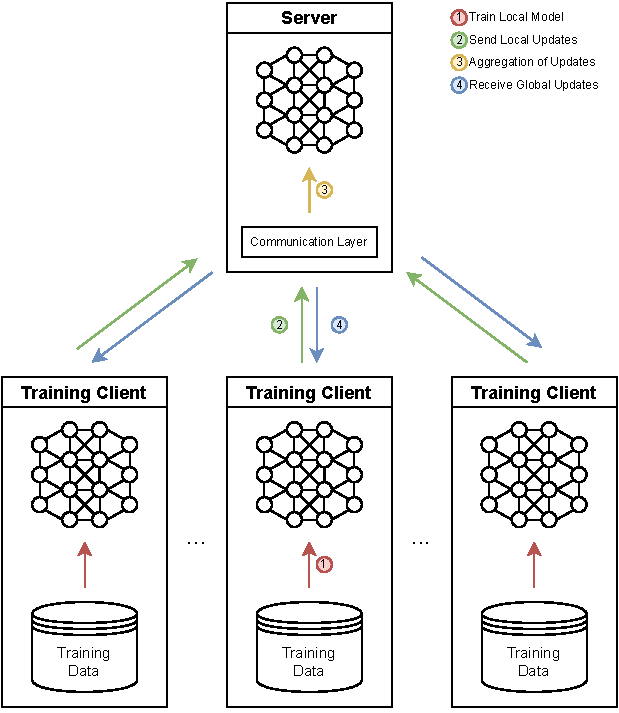
\includegraphics[width=0.6\textwidth]{graphics/hfl-architecture.pdf}
    \caption{Horizontal Federated Learning Architecture}
    \label{fig:hfl_arch}
\end{figure}

In \textit{Horizontal Federated Learning} (HFL), clients with the same data structure collaborate to build a single model. In other words, the different data sets in the different clients share the same feature space, but not the sample space. For example, two banks have similar businesses (feature space), but target different clients (sample space). The architecture of HFL, depicted in \autoref{fig:hfl_arch}, consists of multiple clients training a model, while the central server performs the aggregation of all local updates.

In \textit{Vertical Federated Learning} (VFL), clients share an intersecting sample space, but different feature spaces. For example, two companies operating in the same city have a similar client base (sample space), but different areas of operation (feature space). The architecture of VFL, depicted in \autoref{fig:vfl_arch}, is similar to the one of HFL. However, it includes an additional step to calculate the Private Set Intersection (PSI) since the clients do not share the exact same sample space.

\begin{figure}[!ht] % !ht
    \centering
    \centering
    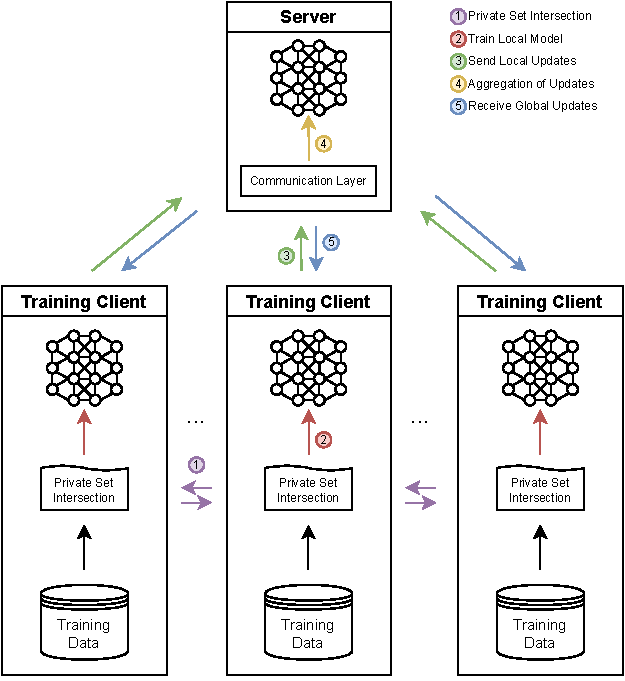
\includegraphics[width=0.6\textwidth]{graphics/vfl-architecture.pdf}
    \caption{Vertical Federated Learning Architecture}
    \label{fig:vfl_arch}
\end{figure}

\section{Blockchain}\label{background:blockchain}

A blockchain is an immutable distributed ledger of transactions maintained by several computers, also known as nodes, linked through a peer-to-peer network. The concept of blockchain was first introduced by Stuart Haber and W. Scott Stornetta in 1991 \cite{10.48550/ARXIV.1810.06130}, being popularized by Satoshi Nakamoto in 2008 with the introduction of the cryptocurrency Bitcoin \cite{nakamoto2009bitcoin}.

\begin{figure}[h]
    \centering
    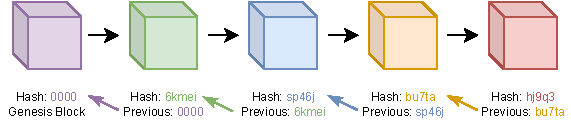
\includegraphics[width=0.8\textwidth]{graphics/blockchain.pdf}
    \caption{Blockchain Representation}
    \label{fig:blockchain_blocks}
\end{figure}

In a blockchain, the data is structured as blocks, as can be seen in \autoref{fig:blockchain_blocks}. Each block contains a certain amount of transactions and links to the previous block via a cryptographic hash, forming a chain. Hence, blockchain. This guarantees fidelity and trust without requiring a trusted third party, which is why it is called a \textit{trustless} system. In addition, since the record is immutable and decentralized, all transactions can be transparently viewed by others.

As mentioned beforehand, a blockchain is maintained by several nodes in a peer-to-peer network. As transactions come in, nodes compete in order to generate the next block. Since it is a decentralized process, multiple nodes will try to create the next block of the chain in parallel. In order to reach an agreement between the nodes, a consensus algorithm is used. The consensus algorithm allows to reach an agreement between multiple decentralized nodes without requiring a singular node to be in charge.

\begin{figure}[h]
    \centering
    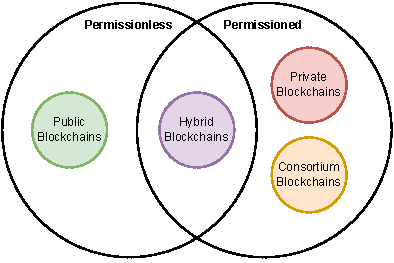
\includegraphics[width=0.5\textwidth]{graphics/blockchain-types.pdf}
    \caption{Blockchain Types}
    \label{fig:blockchain_types}
\end{figure}

There are four different types of blockchain: public, private, consortium and hybrid. Some of these are permissionless, which means that anyone can join the network, while some are permissioned, which means that only allowed parties can join the network. This separation can be visualized in \autoref{fig:blockchain_types}. They work as follows:

\begin{itemize}
    \item \textit{Public Blockchains}. They sit on the permissionless end of the spectrum and therefore anyone can join and participate in the network. There is no central authority.

    \item \textit{Private Blockchains}. In opposition to public blockchains, private blockchains sit on the opposite side of the spectrum, being a permissioned blockchain with a single central authority. This blockchains can only be accessed by allowed parties and they are usually used within organizations.

    \item \textit{Consortium Blockchains}. Similarly to private blockchains, consortium blockchains are also permissioned. However, instead of being controlled by a single authority, they are controlled by a group of different authorities.

    \item \textit{Hybrid Blockchains}. The hybrid blockchains have features of both permissioned and permissionless blockchain systems. On one hand, they are usually controlled by a single authority. On the other hand, they have a mixed usage of permissioned and permissionless protocols running in parallel for different use cases.
\end{itemize}

\subsection{Smart Contracts}

Some blockchain platforms, such as Ethereum \cite{wood2014ethereum}, provide functionality for smart contracts. Smart contracts are small computer programs that live within the blockchain and automatically run when predetermined conditions are met. As they live in the blockchain, they are trustless and are typically used to automate the execution of agreements. This way, every party involved in the agreement is certain that it will be honored once the conditions of the agreement are met.

\subsection{Blockchain Platforms}\label{background:blockchain_platforms}
 
As explained in \autoref{background:blockchain}, blockchain platforms allow developers to build applications on top of blockchain technologies. Even though all platforms are based on the concept of blockchain, they all have different characteristics and restrictions, as well as different sets of features.

As can be seen in \autoref{tab:blockchain_platforms}, around half of the implementations used an already existing platform, where the remaining preferred to implement their own blockchain platform Among already existing platforms, Ethereum was the most popular. When implementing a custom platform, it is easier to overcome certain restrictions such as limits on data per block \cite{8733825, 9524833}.

\begin{table}[!ht]
\centering
\caption{Blockchain Platforms}
\label{tab:blockchain_platforms}
\begin{tabular}{c|c|c|c|c|c}
\hline \hline
                                    & Ethereum      & Hyperledger   & EOS           & MultiChain    & Custom        \\ \hline \hline
\cite{10.1145/3319535.3363256}      & \checkmark    &               &               &               &               \\ \hline
\cite{8905038}                      &               &               &               &               & \checkmark    \\ \hline
\cite{10.48550/arxiv.2011.07516}    & \checkmark    &               &               &               &               \\ \hline
\cite{9524833}                      &               &               &               &               & \checkmark    \\ \hline
\cite{10.48550/arxiv.2101.03300}    &               &               &               &               & \checkmark    \\ \hline
\cite{9159643}                      & \checkmark    &               &               &               &               \\ \hline
\cite{10.1145/3422337.3447837}      & \checkmark    & \checkmark    &               &               &               \\ \hline
\cite{FANG20221}                    &               &               &               &               & \checkmark    \\ \hline
\cite{9184854}                      &               &               &               &               & \checkmark    \\ \hline
\cite{8733825}                      &               &               &               &               & \checkmark    \\ \hline
\cite{8893114}                      &               &               &               &               & \checkmark    \\ \hline
\cite{9274451}                      & \checkmark    &               &               &               &               \\ \hline
\cite{8843900}                      &               &               &               &               & \checkmark    \\ \hline
\cite{8998397}                      &               &               &               &               & \checkmark    \\ \hline
\cite{10.48550/arxiv.2009.09338}    &               &               &               &               & \checkmark    \\ \hline
\cite{8892848}                      &               &               &               &               & \checkmark    \\ \hline
\cite{8945913}                      &               &               & \checkmark    &               &               \\ \hline
\cite{10.48550/arxiv.2202.02817}    &               & \checkmark    &               &               &               \\ \hline
\cite{10.48550/arxiv.2007.03856}    & \checkmark    &               &               &               &               \\ \hline
\cite{10.48550/arxiv.1910.12603}    & \checkmark    &               &               &               &               \\ \hline
\cite{Peyvandi2022}                 & \checkmark    &               &               &               &               \\ \hline
\cite{app8122663}                   & \checkmark    &               &               & \checkmark    &               \\ \hline
\cite{baffle}                       & \checkmark    &               &               &               &               \\ \hline
\cite{9006344}                      & \checkmark    &               &               &               &               \\ \hline
\cite{8894364}                      &               &               &               &               & \checkmark    \\ \hline
\cite{demo}                         &               & \checkmark    &               &               &               \\ \hline
\cite{9233457}                      & \checkmark    &               &               &               &               \\ \hline
\end{tabular}
\end{table}

In this work, we focus on already existing blockchain platforms that do not require internal changes to make the system work. As can be seen in the table, the most common blockchain platform among the reviewed works is Ethereum. Ethereum will also be our platform of choice as it is popular and compatible with all the techniques we are comparing.

\subsection{Consensus Algorithm}\label{background:consensus_algorithms}

The consensus algorithm is one of the most important properties of a Blockchain platform, as it makes it possible for the decentralized blockchain nodes to reach an agreement on what block comes next. In this work, we compare Proof of Work, Proof of Authority and a Byzantine Fault Tolerance-based consensus algorithm.

\begin{itemize}
    \item The PoW consensus algorithm was first introduced in the context of blockchain platforms by Satoshi Nakamoto in Bitcoin \cite{nakamoto2009bitcoin}. PoW works by means of computation effort proofs, where a set of virtual miners race in solving a complex, yet feasible, mathematical problem. The winner of the race generates a cryptographic proof based on the solution of the problem that can be easily verified by others. Then, the winner adds a new block containing the newly verified transactions to the blockchain. In addition, the winner is rewarded according to some pre-determined rules.
    
    \item The PoA consensus algorithm is a reputation-based consensus algorithm that is most commonly used in private blockchain networks. In this system, there is a set of validator nodes that are responsible for validating the new transactions that stake their own reputation. In addition, the validators are known trusted entities that are manually chosen by the network owner.

    \item The IBFT \cite{10.48550/arxiv.2002.03613} consensus algorithm is similar to the Practical Byzantine Fault Tolerance algorithm, which is a three-phase protocol that allows a network with $3f+1$ nodes, where $f$ is the maximum amount of faulty nodes, to reach consensus. The different between IBFT and PBFT is that in the first the set of validators is dynamic, while on PBFT it is static. The network reaches a consensus once $2f+1$ nodes agree.
\end{itemize}

\section{Blockchain-based Federated Learning}\label{background:bfl}

Recently, the idea of applying blockchain to Federated Learning has emerged. This is motivated by the fact that FL architectures are highly dependent on a single central server, leading to a central point of failure, that can be either overloaded or compromised.

\todo{Explain: say there are 3 types of architecture (\cite{10.48550/arxiv.2110.02182}) and that we picked flexibly coupled because it provides the most flexibility?}

\subsection{Participants Selection Techniques}

For the participants selection technique, only random selection and first come, first served-basis selection will be compared. In the former, both the amount of participants and the participants themselves are selected randomly before the start of each round. In the latter, each participant takes initiative to register for the the next round. Once the limit is reached, no more participants are allowed.

\subsection{Scoring and Aggregation Techniques}
\label{background:scoring}

\todo{Mention rewards and why scoring mechanisms can also be used for those}

Scoring techniques attribute a score to each submission and may, or not, influence how the aggregation is made. By default, the aggregation algorithm used is the Federated Averaging algorithm, which can be found in \autoref{eq:fedavg}. In this section, we explain briefly how each of the scoring techniques that will be compared works and if they influence the aggregation algorithm.

\subsubsection{BlockFlow Score}

The BlockFlow scoring algorithm work by giving each submission a score and, based on that score, do the aggregation \cite{10.48550/arxiv.2007.03856}. In this algorithm, each client $a$ gives each other client $k$ a score $s_{a,k} \in [0.0, 1.0]$, which can be based on $a$'s validation set accuracy using $k$'s submission. Based on this scores, a median score and an evaluation quality scores are calculated. The overall scores will then be the minimum between the scaled median score and the scaled least accurate evaluation score.

With the final scores, the aggregation is calculated using the scores as weights in the Federated Averaging algorithm, instead of the number of samples. More details regarding the algorithm specifics can be found in the original paper.

\subsubsection{Marginal Gain Score}

The marginal gain score, also known as contributivity score, is calculated by summing the marginal performance gains of all the client's submissions so far \cite{10.48550/arxiv.2011.07516}. Similarly to BlockFlow scoring, each client has to give each other clients' submission a score. The formula of the client $c$'s submission score $S(c)$ is calculated as follows:

\begin{equation}
    \label{eq:marginal-gain}
    S(c)= \sum_r(v(M_r)-v(M^c_{r+1}))
\end{equation}

Where $v$ is a performance metric, such as accuracy, and $m$ is the model and $r$ the round. These scores are used as weights in the Federated Averaging Algorithm. If the submission's score is equal or below $0$, the submission is ignored.

\subsubsection{Multi-KRUM Score}

The Multi-KRUM algorithm works by giving each submission a score and eliminating dubious submissions based on their score \cite{9170559, Peyvandi2022, 9292450}. This scores are calculated by the servers and are based on the Euclidean distances between the different client $c$'s submissions. The score of each client is denoted as $S(c)$ and calculated as follows:

\begin{equation}
    \label{eq:multi-krum}
    S(c)=\sum_{c \rightarrow k} || \Delta w_c - \Delta w_k|| ^2
\end{equation}

Where $\Delta w$ is a submission and $c \rightarrow k$ are the clients $k$ whose submission $\Delta w_k$ are the $R-f-2$ closest to $\Delta w_c$. In this formula, $R$ is the total number of submissions, while $f$ represents the amount of Byzantine clients. After giving each submission a score, the $R-f$ clients with the lowest scores are chosen and the remaining are rejected. Please note that Byzantine fault tolerant systems behave correctly when no more than $f$ out of $3f+1$ replicas fail.

\subsection{Data Partition and Distribution}

\todo{Fit this better}

Regarding data partition, as can be seen in \autoref{tab:data_distribution}, the vast majority of the literature related to BFL systems has focused on Horizontal Federated Learning systems, with only one focusing on Vertical Federated Learning and none addressing Transfer Federated Learning.

When it comes to data distribution, most of the reviewed work assumed it to be \textit{iid}, while only a minority assuming the data is \textit{non-iid}. Other papers were reviewed, however this information was not specified.

\begin{table}[ht]
\centering
\caption{Data Distribution, Data Partition and Datasets}
\label{tab:data_distribution}
\begin{tabular}{c|c|c|c}
\hline \hline
                                    & Data Distribution & Data Partition & Dataset                            \\ \hline \hline
\cite{10.1145/3319535.3363256}      & I                 & H              & Breast Cancer Dataset              \\ \hline
\cite{8905038}                      & N                 & H              &                                    \\ \hline
% \cite{10.48550/arxiv.2011.07516}    & --                & --             & MNIST                              \\ \hline
\cite{9524833}                      & N                 & --             & --                                 \\ \hline
\cite{9127823}                      & I                 & H              & MNIST, CIFAR10                     \\ \hline
\cite{10.48550/arxiv.2101.03300}    & --                & H              & MNIST                              \\ \hline
\cite{9159643}                      & I                 & H              & MovieLens                          \\ \hline
\cite{10.1145/3422337.3447837}      & I, N              & --             & --                                 \\ \hline
\cite{9223754}                      & I                 & H              & MNIST                              \\ \hline
\cite{FANG20221}                    & --                & H              & CIFAR10                            \\ \hline
\cite{9399813}                      & I                 & H              & MNIST                              \\ \hline
\cite{9184854}                      & --                & H              & --                                 \\ \hline
\cite{8851649}                      & I                 & H              & MNIST                              \\ \hline
\cite{8994206}                      & I                 & H              & MNIST                              \\ \hline
\cite{8733825}                      & I                 & H              & --                                 \\ \hline
\cite{8893114}                      & N                 & H              & MNIST                              \\ \hline
\cite{9274451}                      & N                 & H              & MNIST                              \\ \hline
\cite{9293091}                      & I                 & H              & FEMNIST                            \\ \hline
\cite{8843900}                      & I                 & H              & Reuters, 20News                    \\ \hline
\cite{8998397}                      & I                 & H              & Uber Pickups, MNIST                \\ \hline
\cite{9311394}                      & I                 & H              & MNIST                              \\ \hline
\cite{9170905}                      & I                 & H              & CIFAR10                            \\ \hline
\cite{10.48550/arxiv.2009.09338}    & --                & H              & --                                 \\ \hline
\cite{8892848}                      & I, N              & H              & --                                 \\ \hline
\cite{8945913}                      & --                & H              & MNIST                              \\ \hline
\cite{10.48550/arxiv.2202.02817}    & N                 & H              & MNIST, CIFAR10                     \\ \hline
\cite{10.48550/arxiv.2007.03856}    & --                & H              & --                                 \\ \hline
\cite{10.48550/arxiv.1912.04859}    & I, N              & H,V            & --                                 \\ \hline
\cite{10.48550/arxiv.1910.12603}    & I, N              & H              & --                                 \\ \hline
\cite{9321132}                      & I                 & H              & MNIST                              \\ \hline
\cite{Peyvandi2022}                 & N                 & H              & --                                 \\ \hline
\cite{9079513}                      & I                 & H              & --                                 \\ \hline
\cite{app8122663}                   & I                 & H              & CICIDS 2017                        \\ \hline
\cite{9347812}                      & I                 & H              & CIFAR10                            \\ \hline
\cite{9134967}                      & I, N              & H              & MNIST, CIFAR10                     \\ \hline
\cite{baffle}                       & I                 & H              & NYC 2018 Taxi                      \\ \hline
\cite{9210531}                      & I                 & H              & LFW, MNIST, CelebA, CASIA          \\ \hline
\cite{8894364}                      & --                & H              & MNIST                              \\ \hline
\cite{10.48550/arxiv.2112.07938}    & --                & H              & --                                 \\ \hline
\cite{demo}                         & I                 & H              & MNIST                              \\ \hline
\cite{9233457}                      & I                 & H              & Air-Conditioning                   \\ \hline
\cite{9170559}                      & I                 & H              & MNIST                              \\ \hline
\cite{pirate}                       & I                 & H              & --                                 \\ \hline
\end{tabular}
\caption*{I: IID, N: Non-IID, H: Horizontal, V: Vertical}
\end{table}

\subsection{Differential Privacy}

\todo{Explain local differential privacy, say there are other privacy mechansism, such as homomorphic encryption, smc, etc}
